
\documentclass[tikz,border=2pt]{standalone}
\usepackage{tikz}
\usepackage{amsmath}
\usetikzlibrary{arrows,automata,positioning,calc,decorations.pathmorphing,shapes.geometric}
\begin{document}
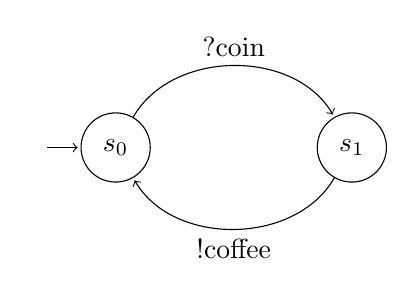
\begin{tikzpicture}
[shorten >=1pt,node distance=2cm,on grid,auto]
      \node[]               (init) {};
      \node[state] (s0) [right=1cm of init] {$s_0$};
      \node[state] (s1) [right=3cm of s0] {$s_1$};

      \path[->]
      (init) edge node {} (s0)
      (s0) edge[loop, out=60, in=120, distance=1cm] node[anchor=south] {\text{?coin}} (s1)
      (s1) edge[loop, out=-120, in=-60, distance=1cm] node[anchor=north] {\text{!coffee}} (s0)
      ;
    
\end{tikzpicture}
\end{document}
